\section{Randlinie \dcsecondauthorshort} \label{ssec:fahrspurerkennung:riverflow:randlinie}
Dieser Abschnitt erklärt den final zur Detektion der Randlinien genutzten Riverflow-Algorithmus. Es wird auf die iterative Methode zur Extraktion der Fahrbahnmarkierung selbst, sowie die Ermittlung der dafür benötigten Startpunkte eingegangen. Weiterhin werden Besonderheiten während der ersten zwei Aufrufe der Funktion sowie Bedingungen zum Terminieren des Algorithmus diskutiert. 
%Er besteht aus den wesentlichen drei Schritten der Startpunktgewinnung, dem Finden von Markierungspunkten mittels Scanlinien und der abschließenden Verifikation der gefundenen Punkte.
\subsection{Startpunktgewinnung}
\label{sssec:fahrspurerkennung:riverflow:randlinie:startpunktgewinnung}
Um den eigentlichen Riverflow-Algorithmus ausführen zu können, wird die ungefähre Lage der seitlichen Fahrbahnmarkierungen in der Nähe des Fahrzeugs benötigt. Zur Ermittlung dieser gibt es 3 Möglichkeiten:
\begin{enumerate}
\item \label{item:solidline:startpoints:dashedline}
Die Bestimmung durch Orientierung und Position des ersten vor dem Fahrzeug gelegenen Mittellinienelementes. Hierzu wird der Mittelpunkt des Elementes senkrecht zu seiner Orientierung um die Fahrspurbreite nach links/rechts verschoben (siehe Abb.~\ref{fig:riverflow:randlinien:startpoints:dashedline}).
\item \label{item:solidline:startpoints:hough}
Eine eindimensionale Hough-Transformation des Bildausschnittes direkt vor dem Fahrzeug wie in Abschnitt~\ref{ssec:grundlagen:hough:vereinfachte} beschrieben (siehe Abb.~\ref{fig:riverflow:randlinien:startpoints:hough}). 
\item \label{item:solidline:startpoints:fixed}
Annahme einer festen Position vor dem Fahrzeug/im Kamerabild.
\end{enumerate}

Die Verfahren \ref{item:solidline:startpoints:hough} oder \ref{item:solidline:startpoints:fixed} werden nur genutzt, wenn die Herangehensweisen \ref{item:solidline:startpoints:dashedline} bzw. \ref{item:solidline:startpoints:dashedline} und \ref{item:solidline:startpoints:hough} kein Ergebnis lieferten.

\begin{figure}[htbp]
	\centering
	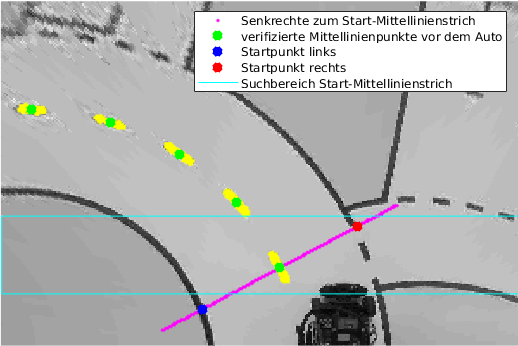
\includegraphics[width=0.75\textwidth]{fahrspurerkennung_riverflow_startpunkte_normal}
	\caption{Startpunktdefinition des Riverflow-Algorithmus für die Randlinien anhand der mittleren Fahrbahnmarkierung}
	\label{fig:riverflow:randlinien:startpoints:dashedline}
\end{figure}

\begin{figure}[htbp]
	\centering
	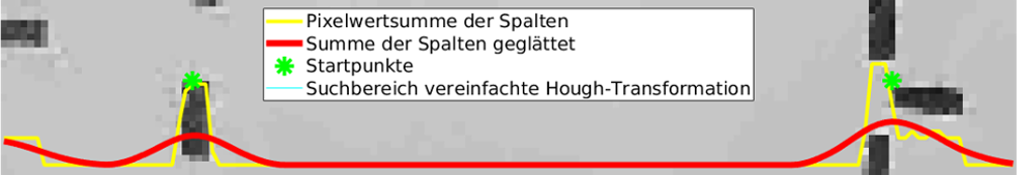
\includegraphics[width=0.75\textwidth]{fahrspurerkennung_riverflow_startpunkte_hough}
	\caption{Startpunktdefinition des Riverflow-Algorithmus für die Randlinien durch eindimensionale Hough-Transformation}
	\label{fig:riverflow:randlinien:startpoints:hough}
\end{figure}

\begin{figure}[htbp]
  \centering
  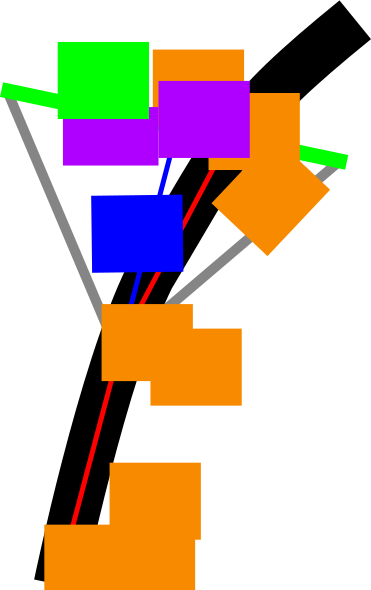
\includegraphics[width=0.3\textwidth]{riverflow_randlinie_prinzip}
  \caption{Funktionsweise des Riverflow-Algorithmus}
  \label{fig:riverflow:randlinie:prinzip}
\end{figure}

\subsection{zentraler Algorithmus}
\label{sssec:fahrspurerkennung:riverflow:randlinie:zentraler_algorithmus}
Die Idee zum im folgenden Abschnitt dargelegten Ansatz zur Verfolgung durchgängiger Fahrbahnmarkierungen entstand auf Basis von \autocite{drauschkeEchtzeitfaehigeStartpunktalgorithmenFuer2016} sowie \autocite{limRiverFlowLane2012}.
Durch Nutzung der Eigenschaften \ref{item:riverflow:rule:solidline} und  \ref{item:riverflow:rule:curvature} kann ausgehend von der aktuellen Linienorientierung in einem bestimmten Kegel (graue Linien in Abb.~\ref{fig:riverflow:randlinie:prinzip}), dessen Öffnungswinkel durch die maximale Krümmung der Fahrspur definiert ist, der weitere Verlauf der Fahrbahnmarkierung angenommen werden.
Algorithmisch genutzt wird dieses Wissen durch die Verwendung der aus Abschnitt~\ref{ssec:fahrspurerkennung:kalman:messung} bekannten Scanlines.
Ausgehend vom letzten gefundenen Punkt der Linie \pnt{p_{n}} wird selbiger um den Vektor \vct{\gls{lat:dv}_n} weiterverschoben und bildet den Mittelpunkt  \pnt{m_{n+1}} der nächsten Scanline \eqref{eq:riverflow:solidline:scanlinemidpoint}. Der Verschiebungsvektor \vct{\gls{lat:dv}_n} wird auf Basis des vorletzten (\pnt{p_{n-1}}) und letzten gefundenen Punktes (\pnt{p_{n}}) der Fahrbahnmarkierung gebildet \eqref{eq:riverflow:solidline:dispvec}. Er stellt den normierten, mit der gewünschten Verschiebungslänge \scl{l_v} multiplizierten Vektor zwischen (\pnt{p_{n-1}}) und (\pnt{p_{n}}) dar.
\begin{equation}
\label{eq:riverflow:solidline:dispvec}
\vct{\gls{lat:dv}_n} =  \frac{\pnt{p_{n}} - \pnt{p_{n-1}}}{\nrm{\pnt{p_{n}} - \pnt{p_{n-1}}}} \cdot \scl{l_v}
= 
\begin{pmatrix}
\scl{d_{nx}} \\
\scl{d_{ny}}
\end{pmatrix}
\end{equation}
\begin{equation}
\label{eq:riverflow:solidline:scanlinemidpoint}
\pnt{m_{n+1}} =  \pnt{p_n} + \vct{\gls{lat:dv}_n}
\end{equation}
Mithilfe des zu \vct{\gls{lat:dv}_n} \eqref{eq:riverflow:solidline:dispvec} senkrechten Richtungsvektors \vct{l_{n+1}} \eqref{eq:riverflow:solidline:scanlinedirectionvec} der \begin{math} (n+1)\end{math}-sten  Scanline \begin{math} \vct{s_{n+1}} \end{math} kann selbige wie folgt beschrieben werden:
\begin{equation}
\label{eq:riverflow:solidline:scanlinecontinous}
\vct{s_{n+1}} =
\pnt{m_{n+1}}  + \alpha \cdot \vct{l_{n+1}}
\qquad \alpha \in \mathbb{R}
\end{equation}
\begin{equation}
\label{eq:riverflow:solidline:scanlinedirectionvec}
\vct{l_{n+1}} =
\begin{pmatrix}
-d_{ny} \\
d_{nx}
\end{pmatrix}
\end{equation}
Der Wertebereich des skalaren Faktors \scl{\alpha} gibt hierbei die Ausdehnung der Scanline um ihren Startpunkt/Mittelpunkt \pnt{m_{n+1}} herum an.

Da die Filterantwort des Kantendetektors für das gesamte Bild bereits vorliegt, um die Mittellinie detektieren zu können, kann auch zur Erkennung der seitlichen Fahrbahnmarkierung auf diese zurückgegriffen werden. Bei der nun folgenden, in Abschnitt~\ref{ssec:fahrspurerkennung:kalman:messung} ausführlich beschriebenen Extraktion von zentral auf der Fahrbahnmarkierung liegenden Punkten, entfällt also die Notwendigkeit der Filterung. Da der Riverflow-Algorithmus sich im Bildkoordinatensystem \gls{lat:BildKOS} bewegt, ist auch die in Passage~\ref{ssec:fahrspurerkennung:kalman:messung} notwendige Hin- und Rücktransformation vom bzw. zum Linienkoordinatensystem \gls{lat:LinienKOS} nicht notwendig. In allen anderen Punkten gleicht der Weg von der aufgestellten Scanline \vct{s} zu den darauf ermittelten, zentral in der Fahrbahnmarkierung liegenden Koordinaten \vct{p} dem in Abschnitt~\ref{ssec:fahrspurerkennung:kalman:messung} dargelegten.

%Hierfür wird die Scanline in eine diskrete Koordinatenserie überführt \ref{eq:riverflow:solidline:scanlinediscrete}, deren Elemente auf ganzzahlige Werte gerundet werden.
%\begin{equation}
%\label{eq:riverflow:solidline:scanlinediscrete}
%\pnt{s_{{n+1}_d}} =
%\pnt{m_{n+1}}  + z \cdot \vct{l_{n+1}} 
%\qquad z \in \mathbb{Z}
%\end{equation}
%Die durch die Koordinatenserie adressierten Pixel der Filterantwort können nun zur weiteren Verarbeitung in einen Zeilenvektor geschrieben werden. 
% \begin{equation}
% \vct{f} =
% \begin{pmatrix}
% \scl{f_1} & \scl{f_2} & \dots & \scl{f_i} & \dots & \scl{f_n}
% \end{pmatrix}
% \end{equation}
%Nun wird \mxm{\vct{f}} ermittelt. Ist \mxm{\vct{f}} größer als ein bestimmter Schwellwert \scl{s}, wird der Index \begin{math} i_{max} \end{math} des Maxima in \vct{f} vorgemerkt. Um eine Linie nicht wiederholt zu finden, muss die in \vct{f} verbleibende, durch dieselbe Markierung verursachte Filterantwort entfernt  werden.
%\begin{equation}
%\scl{f_{i_{max}-\text{Linienbreite}/2}} \dots \scl{f_{i_{max}}} 
% \dots  \scl{f_{i_{max}+\text{Linienbreite}/2}} = 0
% \end{equation}
%Darauffolgend kann nach weiteren \scl{s} überschreitenden Einträgen in \vct{f} gesucht und wie mit dem ersten \mxm{\vct{f}} verfahren werden.
%Wird kein ausreichend großes \mxm{\vct{f}} mehr gefunden, können den gefundenen Indizes \begin{math} i_{max} \end{math} via \eqref{eq:riverflow:solidline:scanlinediscrete} Koordinaten \pnt{p_{n+1}} zugeordnet werden.

Sind mehrere auf der Scanline \vct{s_{n+1}} gefundene Punkte  \pnt{p_{n+1}} vorhanden, so werden ab diesem Zeitpunkt multiple Hypothesen einer seitlichen Fahrbahnmarkierung verfolgt.
Jetzt kann die nächste Iteration des Riverflow-Algorithmus mit der Bildung des folgenden Verschiebungsvektors bzw. der folgenden Verschiebungsvektoren \vct{\gls{lat:dv}_{n+1}} starten.

\subsection{Sonderfall 1. und 2. Iteration}
Da in der 1. und 2. Iteration keine Punkte \pnt{p_{n-1}} und \pnt{p_n} vorhanden sind, muss der Verschiebungsvektor \gls{lat:dv} anderweitig bestimmt werden. 
Wurde der Startpunkt wie in Methode~\ref{item:solidline:startpoints:dashedline} beschrieben durch ein Mittellinienelement bestimmt, kann dessen Orientierung als Richtung des Verschiebungsvektors genutzt werden.
Bei den Verfahren \ref{item:solidline:startpoints:hough} und \ref{item:solidline:startpoints:fixed} wird eine konstante Verschiebung in Fahrtrichtung des Fahrzeugs genutzt.

\subsection{Ende des Algorithmus}
\label{sssec:fahrspurerkennung:riverflow:randlinie:ende} 
Der Algorithmus wird beendet, sobald:
\begin{enumerate}
\item  
Der Mittelpunkt \begin{math} \vct{m}  \end{math} der nächsten Scanline außerhalb des Bildbereichs liegt
\item \label{item:fahrspurerkennung:riverflow:randlinie:ende:keinpunkt}
Auf der aktuellen Scanline keine zentral in der Fahrbahnmarkierung liegenden Koordinaten \vct{p} gefunden wurden. Vor dem endgültigem Abbruch der Verfolgung einer Fahrbahnmarkierung wird der Verschiebungsvektor \vct{\gls{lat:dv}} der ergebnislosen Scanline verlängert und die erneute Suche nach einer ausreichend großen Filterantwort durchgeführt, somit können auch kleine Unterbrechungen einer Linie überwunden werden.
\item 
Die betragsmäßige Orientierungsänderung \(\btr{\scl{\Delta \phi}} = \btr{\atantwo{\scl{r_{n+1 y}, r_{n+1 x}}} \linebreak - \atantwo{\scl{r_{n y}, r_{n x}}}}\) der zwei Vektoren \(\vct{r_{n+1}}=\vct{p_{n+1}}-\vct{p_{n}}\) sowie \(\vct{r_{n}}=\vct{p_{n}}-\vct{p_{n-1}}\) zwischen den letzten zwei gespeicherten und dem gerade gefundenen Punkt einen Grenzwert überschreitet (s. Abb.~\ref{fig:riverflow:randlinie:prinzip}). Da der Straßenverlauf im gegebenen Szenario niemals abknickt, wäre dies ein sicheres Zeichen einer Fehlerkennung. Diese Abbruchbedingung ließe sich auch durch Die Länge der Scanlines einstellen, indem somit der Öffnungswinkel des Suchkegels (graue Linien in Abb.~\ref{fig:riverflow:randlinie:prinzip}) reduziert wird und Punkte, die zu einem Abknicken der erkannten Fahrbahnmarkierung führen, gar nicht erst erkannt werden. 
Die Prüfung der Orientierungsänderung wird jedoch beim in Abschnitt~\ref{sssec:fahrspurerkennung:riverflow:randlinie:gestrichelt} beschriebenen Sonderfall der Extraktion des Punktes \vct{p_{n+1}} notwendig.
\end{enumerate}

\begin{figure}[htbp]
  \centering
  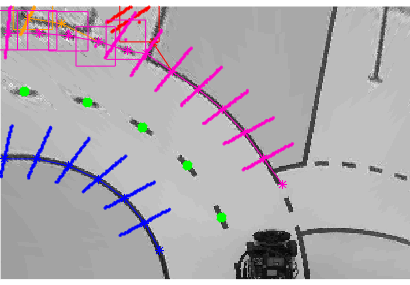
\includegraphics[width=0.75\textwidth]{riverflow_randlinien_komplett}
  \caption[Plot eines Riverflow-Durchlaufs für die Randlinien]{Plot eines Riverflow-Durchlaufs für die Randlinien: \par Die Farben Rot, Orange und Pink stellen die Hypothesen der rechten, Blau die einzige Hypothese der linken Fahrbahnmarkierung dar. Diese Hypothesen bestehen jeweils aus den * für gefundene Punkte, dünnen Linien für deren Verschiebungsvektoren zueinander, fettgedruckten Geraden zur Darstellung der Scanlines sowie Scanquadraten und deren Mittelpunkte (\(\cdot\)) im Bereich der unterbrochenen Markierung. Die grünen Punkte repräsentieren die bereits erkannten \& verifizierten Mittellinienpunkte. }
  \label{fig:riverflow:randlinien:plot_komplett}
\end{figure}
